\begin{scriptsize}

\begin{multicols}{2}
\section{Realisierungs-Methoden}
\subsection{ROM}
Mit einem ROM lassen sich rein kombinatorische Schaltungen in Form einer Look-Up-Table realisieren.
\begin{itemize}
	\setlength{\itemsep}{1pt}
  \setlength{\parskip}{0pt}
  \setlength{\parsep}{0pt}
  
	\item Eingangsvariablen = Adresse
	\item Speicherwert = Ausgang (programmierbar)
\end{itemize}
\vfill\null
\columnbreak
\subsection{PLD}
Programmierbares Device aus AND- und OR-Matrix, mindestens eine Matrix programmierbar.
\begin{itemize}
	\setlength{\itemsep}{1pt}
  \setlength{\parskip}{0pt}
  \setlength{\parsep}{0pt}
  
	\item PAL $\rightarrow$ OR-Matrix fest, AND-Matrix programmierbar, Fuses
	\item PLA $\rightarrow$ OR und AND Matrix frei programmierbar, Fuses
	\item GAL $\rightarrow$ Wie PLA plus programmierbare Ausgangsnetzwerke (Tristate), EEPROM
\end{itemize}
SPLD (Simple PLD): F"ur Funktionen die als DNF vorliegen geeignet, heute gr"osstenteils von CPLD und FPGA verdr"angt.
\end{multicols}

\begin{multicols}{2}
\subsection{CPLD (Complex PLD)}
\begin{itemize}
	\setlength{\itemsep}{1pt}
  \setlength{\parskip}{0pt}
  \setlength{\parsep}{0pt}
  
	\item Verbund von PL-Makrozellen, die mit Bussen verbunden sind, Speicherung der Konfiguration in Flash.
	\item Durch regelm"assige Struktur sind Signallaufzeiten vorhersagbar.
	\item Wegen grosser Zahl an Logikbl"ocken sehr gut f"ur parallele Prozesse geeignet.
\end{itemize}
\vfill\null
\columnbreak
\subsection{FPGA}
2D-Array von Logikbl"ocken, die "uber Routing-Kanal und Schaltmatrizen miteinander und mit I/O verbunden werden.
\begin{itemize}
	\setlength{\itemsep}{1pt}
  \setlength{\parskip}{0pt}
  \setlength{\parsep}{0pt}
  
	\item Logikblock (LogicCell) $\rightarrow$ Look-Up-Table mit D-FlipFlop, kann beliebige Funktionen ausführen
	\item Schaltmatrizen $\rightarrow$ programmierbare Verbindungen
	\item Makrozellen $\rightarrow$ Feste Funktionen wie z.B. Memory, Clock Management ...
\end{itemize}
Die Konfiguration wird im RAM gespeichert (flüchtig). D.h. bei jedem Boot muss der Code von einem Festspeicher geladen werden.
\end{multicols}

%\subsection{Xilinx Spartan 3}
%\begin{itemize}
%	\setlength{\itemsep}{1pt}
%  \setlength{\parskip}{0pt}
%  \setlength{\parsep}{0pt}
%
%	\item Logic Cell (LC): Kleinste Einheit, enth"alt LUT mit 4 Eing"angen und eime D-FlipFlop. LUT kann als 16x1 bit SRAM oder Schieberegister 		konfiguriert werden. Zus"atzlich pro LC CarryLogic und MUX.
%	\item Slice: 1Slice = 2 Logic Cell
%	\item Configurable logic bloc (CLB): 1 CLB = 4 Slices = 8 Locic Cells. \\
%	Inerhalb dieser Einheit existieren spezifische Verbindungsstrukturen.
%\end{itemize}
%
%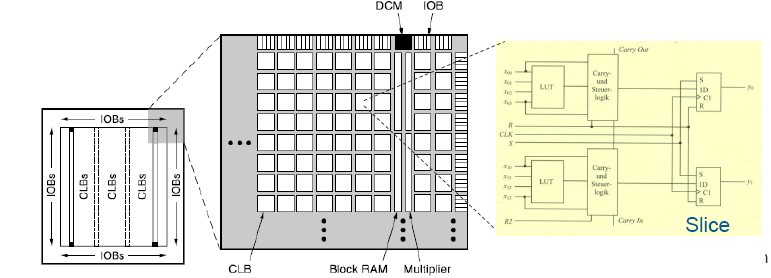
\includegraphics[width=0.8\textwidth]{pics/fpgastruct}

\begin{multicols}{2}
\subsection{Semi-Custom-ASIC}
\begin{itemize}
	\setlength{\itemsep}{1pt}
  \setlength{\parskip}{0pt}
  \setlength{\parsep}{0pt}
  
	\item Mikrozellen aus p- und n-FETs werden durch Verdrahtung zu Gates 			
		$\rightarrow$Gate-Array/Sea of Gates
	\item Gates k"onnen durch Verdrahtungskan"ale verbunden werden.
	\item Standardfunktionen k"onnen mit IP (Intellectual-Property)-Cores implementiert werden.
	\item In Mixed-Signal Arrays sind zus"atzlich spezifische Analogbauteile enthalten.
\end{itemize}	
\vfill\null
\columnbreak	
\subsection{Full-Custom-ASIC}
V"ollig kundenspezifische ASICs, oft werden IP-Cores f"ur Standardfunktionen verwendet. Digitale und analoge Komponenten auf einem IC m"oglich. Voll auf Anwendung anpassbare Eigenschaften (Stromverbrauch, Gr"osse, Geschwindigkeit etc.).
\end{multicols}

\end{scriptsize}

\subsection{Vergleichstabelle}
\begin{minipage}{0.41\textwidth}
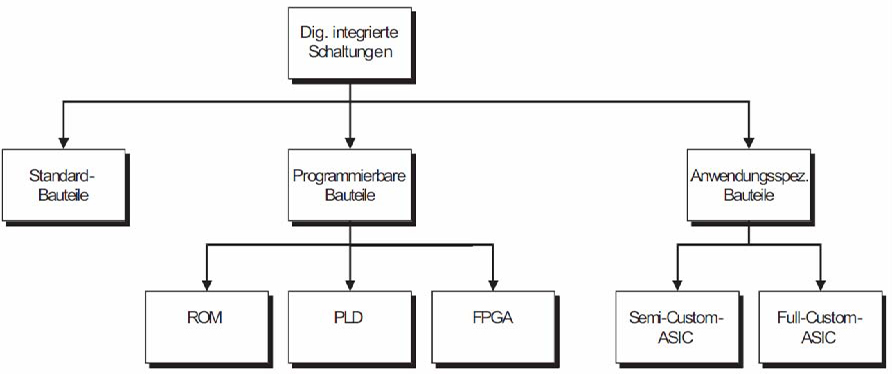
\includegraphics[width=0.99\textwidth]{pics/devicecomparetables}
\end{minipage}
\hfill
\begin{minipage}{0.58\textwidth}
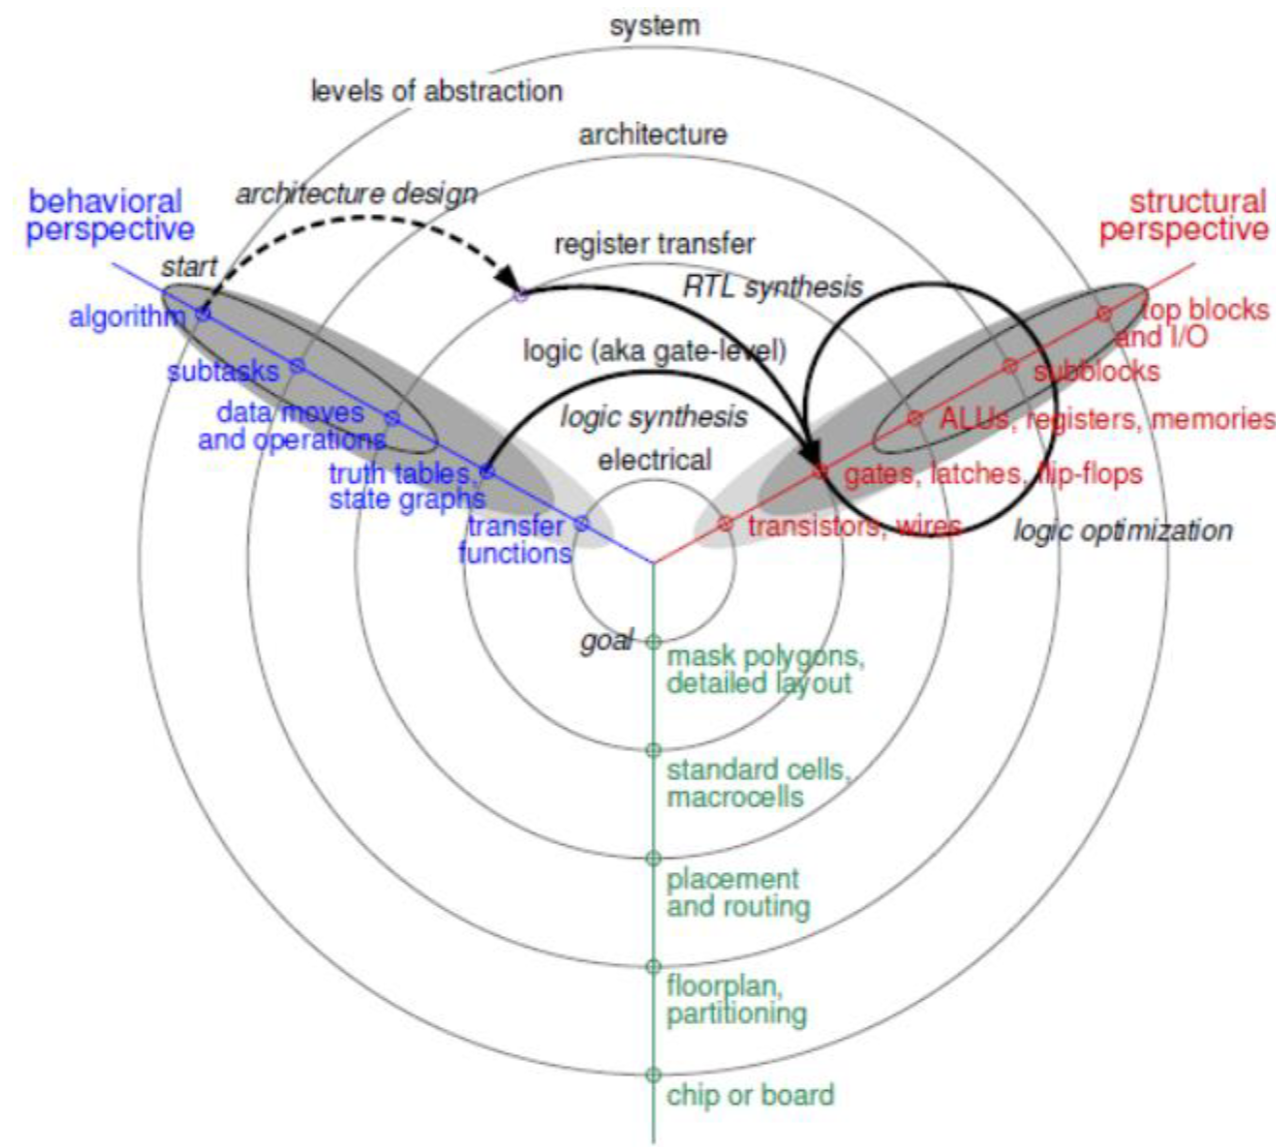
\includegraphics[width=0.7\textwidth]{pics/abstraktion.png}
\end{minipage}

\begin{tabular}{|l|c|c|c|c|c|c|}
	\hline
	Kriterien & Standard Bauteile & ROM & PLD & FPGA & Semi-Custom & Full-Custom \\
	\hline
	Machbarkeit & ++ & - - & - - & + & + & +++ \\
	\hline
	Realisierungszeit & + & ++ & ++ & ++ & - & - - \\
	\hline
	Iterationszeit & - & ++ & ++ & ++ & - & - - \\
	\hline
	NRE (Non Recurring Engineering) & ++ & + & + & + & - & - - -\\
	\hline
	St"uckpreis & - - & + & + & - & + & +++ \\
	\hline
\end{tabular}
	